\documentclass[12pt, a4paper]{article}

% Standard TikZ and modern arrow heads
\usepackage{tikz}
\usetikzlibrary{arrows.meta}

\begin{document}

\section*{UML Class Diagram: Antigravity Engine Software System}

\begin{center}
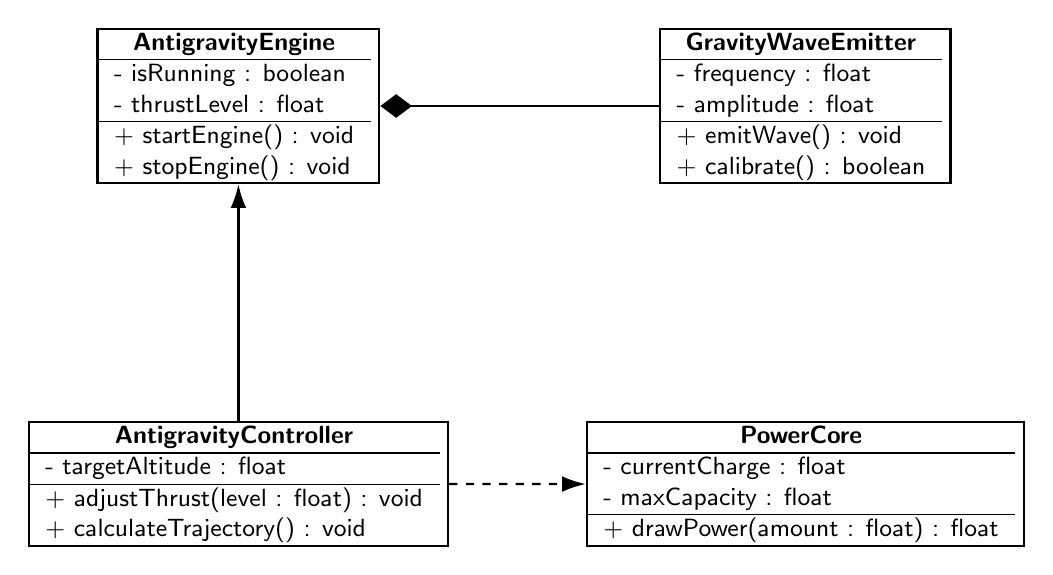
\begin{tikzpicture}[
    xscale=1.2, yscale=1.2,
    every node/.style={font=\small\sffamily},
    classbox/.style={draw, rectangle, fill=white, thick, align=left, inner sep=0pt, font=\small\sffamily}
]

    % --------------------------------------------------------
    % 1. DEFINE CLASSES USING STANDARD TABULARS
    % --------------------------------------------------------

    % AntigravityEngine Class
    \node (engine) [classbox] at (0, 0) {
        \begin{tabular}{l}
        \multicolumn{1}{c}{\textbf{AntigravityEngine}} \\ \hline
        - isRunning : boolean \\
        - thrustLevel : float \\ \hline
        + startEngine() : void \\
        + stopEngine() : void
        \end{tabular}
    };

    % GravityWaveEmitter Class
    \node (emitter) [classbox] at (6, 0) {
        \begin{tabular}{l}
        \multicolumn{1}{c}{\textbf{GravityWaveEmitter}} \\ \hline
        - frequency : float \\
        - amplitude : float \\ \hline
        + emitWave() : void \\
        + calibrate() : boolean
        \end{tabular}
    };

    % AntigravityController Class
    \node (controller) [classbox] at (0, -4) {
        \begin{tabular}{l}
        \multicolumn{1}{c}{\textbf{AntigravityController}} \\ \hline
        - targetAltitude : float \\ \hline
        + adjustThrust(level : float) : void \\
        + calculateTrajectory() : void
        \end{tabular}
    };

    % PowerCore Class
    \node (powercore) [classbox] at (6, -4) {
        \begin{tabular}{l}
        \multicolumn{1}{c}{\textbf{PowerCore}} \\ \hline
        - currentCharge : float \\
        - maxCapacity : float \\ \hline
        + drawPower(amount : float) : float
        \end{tabular}
    };

    % --------------------------------------------------------
    % 2. DEFINE RELATIONSHIPS
    % --------------------------------------------------------

    % Composition: Engine strictly owns the GravityWaveEmitter.
    % The Diamond sits at the Engine side, so we draw from emitter -> engine
    \draw [-{Diamond[fill=black, length=4mm, width=3mm]}, thick] (emitter) -- (engine);

    % Association: The Controller operates the Engine. (Standard Arrow)
    \draw [-{Latex[length=3mm, width=2mm]}, thick] (controller) -- (engine);

    % Dependency: The Controller depends on the PowerCore. (Dashed Arrow)
    \draw [-{Latex[length=3mm, width=2mm]}, dashed, thick] (controller) -- (powercore);

\end{tikzpicture}
\end{center}

\end{document}
